\chapter{Computational models of analogical reasoning}
\label{CHAP:computational_models_of_analogical_reasoning}
\renewcommand{\contentsname}{Content}
\localtableofcontents*
\vspace*{\baselineskip}

\initial{R}oughly speaking, analogy is a matter of establishing parallels
between two different situations. Reasoning by analogy allows to infer
properties about one of the two situations based on our knowledge of the other.
Closely related to analogical reasoning is the idea of analogical proportion,
which is a statement of the form \textit{a is to b as c is to d}, often written
$a:b::c:d$. Here also, one of the four elements may sometimes be inferred if
the three other are known: this is called the \textit{solving} of the
analogical equation $a:b::c:~?$.

The first two chapters of this document will provide the necessary background
on formal analogical models and especially analogical proportions. In this
first chapter, we provide an overview of various attempts to formalize
analogical reasoning, with a strong emphasis on computational models. In the
next chapter we will describe in more details the modeling of analogical
proportions, especially in the Boolean and real settings and their application
to machine learning tasks. This chapter is structured as follows.

Section \ref{SEC:models_without_proportions} will be devoted to the description
of existing models that do not make explicit use of analogical proportions, and
Section \ref{SEC:models_with_analogical_proportions} will describe models that
make use of analogical proportion in one way or another, but that still do not
use analogical proportions in a formal way (these models will be the object of
the next chapter).

\section{Models without analogical proportions}
\label{SEC:models_without_proportions}

In this first section, we will review some past attempts at modeling analogical
reasoning, where no use is made of analogical proportions.

\subsection{First attempts by P\'olya and Hesse}

In his famous book \textit{How to Solve It} \cite{Pol45}, the mathematician
George P\'olya suggests to his readers various ways of reaching the solution
of mathematical problems. Among the different heuristics that are
proposed, analogy has a prominent place. Considering the problem of finding
the center of gravity of a homogeneous tetrahedron, P\'olya suggests to observe
that the tetrahedron and the triangle have many similar features, and to first
find the center of gravity of the triangle: a somewhat simpler problem. He
writes:

\begin{quote}
Knowing that the triangle and the tetrahedron are alike in many respects, we
  conjecture that they are alike in one more respect. It would be foolish to
  regard the plausibility of such conjectures as certainty, but it would just
  as foolish, or even more foolish, to disregard such plausible conjectures.
\end{quote}

As the center of gravity of a triangle is the meeting point of the three
medians, the analogical argument suggests that the center of gravity of the
tetrahedron is the meeting point of the six median planes. The work of P\'olya
is probably the most elaborated analysis of analogical reasoning as a tool for
problem solving in the modern era. Later in \cite{Pol54}, P\'olya formalizes
this idea in what he calls a \textit{pattern of plausible inference}:
$$
\inferrule{a \text{ is analogous to } $b$ \\\\ a \text{ is true}}{ $b$ \text{
  is more credible} }
$$


Another early attempt at formalizing analogical reasoning is due to the
philosopher of science Mary Hesse. In \cite{Hes66}, Hesse proposes to represent
an analogy in a tabular form, as illustrated in Table \ref{TAB:Hesse_analogy}.
\begin{table}[t]
  \centering
  \begin{tabular}{ll}
    \toprule
    Bovine & Equid\\
    \midrule
    Is mammal & Is mammal\\
    Has hoofs & Has hoofs\\
    Eats grass & Eats grass\\
    $\sim$ 1.6 meters high & $\sim$ 1.6 meters high\\
    Harmless & Harmless\\
    Domesticated & \textit{Domesticable}?\\
    \bottomrule
  \end{tabular}
  \caption{The tabular representation of an analogy between cows and horses.}
  \label{TAB:Hesse_analogy}
\end{table}
We already recognize here a mapping between two domains: a source domain (the
bovine domain) and a target domain (the equid domain). In Hesse's theory, an
analogy should follow three general principles to be considered seriously. The
first (questionable) requirement is the \textbf{requirement of material
analogy}: for Hesse, material similarities (i.e. \textit{observable}
similarities) between the two domains are more important than formal
similarities, which emerge when the two domains can be seen as two different
interpretations of a unifying model. In that sense, Hesse rejects the deep
underlying similarities that may bond the two domains. The second requirement
is that when it comes to inferring a property $Q$ (e.g. \textit{is a horse
domesticable?}), there should be a \textbf{causal relationship} between the
known properties $P$ and the one we need to infer. For example in our example
of Table \ref{TAB:Hesse_analogy}, the fact that the animals are harmless
and that they eat grass probably helps us to domesticate them. Whether they
have hoofs is however fairly irrelevant for the matter. Finally, the \textbf{no
essential difference condition} states that if a property $P$ is causally
related to the hypothetical property $Q$ in the source domain, then it should
also be the case in the target domain. For example if the horse was not
harmless, or if it had a very special dietary regime, then we should probably
not infer that it is easily domesticable.

Let us also briefly mention that in \cite{Hes59}, Mary Hesse outlined a formal
framework allowing to define analogical proportions in a modular lattice,
anticipating quite remarkably other future works that will be reviewed in
Chapter \ref{CHAP:formal_analogical_proportions}.

\subsection{Analogy as a structural mapping}

The role of a structural mapping between a source domain and a target domain
has been recognized for a long time as a key component of analogical reasoning:
see for example P\'olya in \cite{Pol54}, or Hesse's theory that we have just
described. As such, this principle has led to numerous theories and
computational models that we briefly (and non-exhaustively) recall here.

\paragraph{Gentner's Structure Mapping Theory\\}

Probably the most influential model of analogical reasoning is the Structure
Mapping Theory (SMT), introduced by the American cognitive scientist Dedre
Gentner in \cite{Gen83}. The main feature of SMT is to consider that good
analogies are those that result from strong, deep, relations and dependencies
between the source and the target domains, rather than on some superficial
characteristics. In this regard, SMT departs from Hesse's theory in a
significant way.

The point of Gentner is that superficial similarities are often irrelevant,
while what matters in an analogy are the underlying \textbf{structural}, high
order relations between the objects at play. To exemplify, Gentner argues that
when one says that \textit{a battery is like a reservoir}, the analogy stands
because at some abstract level, a battery and a reservoir serve the same
purpose: to release some potential energy that has been stored for some time.
The fact that batteries come in different shapes, colors and sizes than
reservoirs does not play any role in the relevance of the analogy. This
principle is called the \textbf{systematicity principle}, for which we now give
some technical details.

The world is assumed to be represented by objects (belonging either to the
source domain $S$ or to the target domain $T$), along with some
\textbf{predicates} that deal with one or more objects of the same domain. The
distinction is made between predicates that only take one argument
(\textbf{attributes} of objects), and those  that take at least two arguments 
(\textbf{relations}). Higher-order relations are relations for which arguments
are themselves relations, instead of simple objects. To illustrate these
syntactic distinctions, \textit{TALL(Bob)} and \textit{BLONDE(Alice)} are
attributes over the objects \textit{Bob} and \textit{Alice}.
\textit{ARE\_FRIENDS(Bob, Alice)} and \textit{HAVE\_DINNER(Bob, Alice)} are
first-order relations, and \textit{CAUSE[ARE\_FRIENDS(Bob, Alice),
HAVE\_DINNER(Bob, Alice)]} is a second-order relation.

In SMT, an analogy is defined as a one-to-one mapping $M$ from $S$ to $T$ that maps
relations (and only relations) between the two domains. The systematicity
principle mentioned earlier states that during the mapping, attributes of
objects (considered to be superficial features) are discarded and not taken
into account, while higher-order relations are given priority over lower-order
ones. Also, out of two relations of the same order, the one that is the most
involved into other (higher-order) relations is the most likely to be mapped in
the target domain. This last requirement gives an implicit rule to somehow
assess the relevance of a relation in an analogy.

Note that this definition of analogy involves purely structural and syntactical
features. The semantic underlying the relations (or the objects) are completely
out of concern. In our example, the fact that \textit{Alice} and \textit{Bob}
are actually friends is of no importance: for SMT this relation is nothing but
a first-order relation, with no particular meaning. As far as SMT is concerned,
\textit{Alice} and \textit{Bob} could just as well be arch-enemies, it would
not make any difference during a potential mapping process with a target domain
(which would, for example, involve two other individuals with a similar
relationship).

While SMT is a purely theoretical framework for analogy, these ideas have been
practically implemented in a software called the Structure Mapping Engine (SME)
\cite{FalForKenGen89} written in LISP, leading to numerous applications. A
recent example is that of a program that is able to solve Raven's Progressive
Matrices \cite{LovForUsh10}, a typical kind of visual geometric
puzzles. The SME algorithm, in complete accordance with SMT, can be
conceptually summarized as follows:
\begin{enumerate}
    \item Look for all potential matches between relations in the source domain
      and the target domain.
    \item Try to group matches into maximally consistent collections of
      matches.
    \item From each collection, infer some relations that might stand in the
      target domain.
\end{enumerate}
In its most simple form, the SME algorithm can be viewed as the finding of a
maximum common subgraph between two graphs, namely those representing the
source and the target domains. As such, SME is part of the connectionist
approaches.

In  \cite{ChaFreHof92}, authors point out various concerns about SMT and SME.
Among them is the fact that SME is too reliant on the (human-made) description
inputs of the source and target domains, and that the intelligence mostly comes
from these descriptions:

\begin{quote}
  when the program's discovery of the correspondences between the two situations
  is a direct result of its being explicitly given the appropriate structures
  to work with, its victory in finding the analogy becomes somewhat hollow.
  Since the representations are tailored (perhaps unconsciously) to the problem
  at hand, it is hardly surprising that the correct structural correspondences
  are not difficult to find.
\end{quote}

Also, while the systematicity principle is undoubtedly at the core of many
analogies, it should seem natural to challenge it in some other situations. It
is indeed quite easy to find analogies were superficial features are the most
decisive ones \cite{Bar10}.

\paragraph{Prior to SMT: Winston's theory\\}

We should mention that SMT and SME are not the first theory/engine couple that
models analogical reasoning based on the mapping of two situations. Indeed in
\cite{Win80}, Patrick H. Winston already presents a theory along with a
program that also rely on this general view. Winston uses a propositional
representation of the two situations that are extracted from natural language
sentences.

Contrary to SMT, Winston's view of analogy is fairly close to that of Hesse.
For Winston, the matching between the two situations should not only involve
high order relations, but also the attributes of the objects. Moreover, he
acknowledges the importance of \textbf{causal} relations to guide the mapping
process, which is compliant with Hesse's theory. Winston also considers that
the mapping process is \textit{constraint-based}, which probably inspired the
model of Holyoak and Thagard that we describe now.

\paragraph{The Constraint Satisfaction Theory\\}

As some of the most influential theories of analogical reasoning, SMT and
Winston's model have opened the way to various other models such as that of
Holyoak and Thagard \cite{HolTha89}. Here as well, an analogy is considered to
be a mapping between two domains $S$ and $T$\footnote{with the exception that
the mapping goes here from $T$ to $S$.}. Taking over Gentner's systematicity
principle (in a relaxed form), Holyoak and Thagard exhibit two additional
dimensions of importance in an analogical process. First, the semantics behind
the objects at hand, i.e.  the meaning that human agents associate with these
objects, are taken into account. In this theory, the two relations
\textit{ARE\_FRIENDS} and \textit{ARE\_ENEMIES} are not the same. This clearly
stands in contrast with SMT, where all object attributes are simply discarded
(along with their meanings), and seems to be in accordance with Hesse's
requirement of material analogy. Second, this theory also involves the
pragmatic considerations of the human agent: the goal and purpose of the
analogist should somehow guide the mapping process in some direction or
another. Mappings that serve the purpose of the agent are therefore given
higher priority than others.

Another main difference with SMT, where the systematicity principle is a fixed,
inflexible rule, is that here the three dimensions (systematicity, semantic
similarity and pragmaticity) are interpreted as \textbf{constraints} and not as
rigid directions. These constraints are only here to guide the mapping process.

Holyoak and Thagard's theory has been implemented in a LISP software called
ACME (Analogical Constraint Mapping Engine), in a similar fashion as the
Copycat program (detailed later in Section \ref{SEC:copycat}) in that they are
both cooperative algorithms. Much like SME, ACME is part of the connectionist
approaches.

\paragraph{Heuristic-Driven Theory Projection\\}

Another framework where structural mapping is considered at the core of an
analogical process is the so-called Heuristic-Driven Theory Projection proposed
by Gust, K\"uhnberger and Schmid \cite{GusKunSchTCS06}. While in SME and ACME
the main algorithm boils down to finding a maximum common subgraph between the
two domain representations, HDTP banks on a more formal approach. The two
domains are formally described in first-order logic as a set of facts
(variable-less formulas such as \textit{TALL(Bob)}) and a set of laws
(quantified formulas, such as \textit{$\exists x,$ TALL($x$)}). Using an
anti-unification (generalization) process, the two domains (or theories) $S$
and $T$ are mapped through a generalized theory $G$ described in a second-order
logic. As expected from the name of the framework, the way the mapping is
performed is heuristic-based. From this generalized theory, a transfer of
knowledge can be applied to the target domain, thus allowing the inference of
new facts and laws, provided that they are in accordance with the already known
formulas.  This process of generalization followed by a transfer phase is what
is called a \textbf{theory projection}.

\subsection{Logical view of analogical reasoning}
\label{SEC:Davies_and_Russel}

We have seen so far various models of analogical reasoning that mostly rely on
some heuristic. In contrast with this tendency, Davies and Russel
\cite{DavRus87} proposed first order description of the analogical inference
process, and most importantly a set of conditions required for this inference
process to be sound.  Concretely, they provide some sufficient conditions that
must hold on two properties $P$ and $Q$ for the following inference rule to be
valid:
$$\inferrule{P(S) \wedge Q(S) \\\\ P(T)}{Q(T)},$$
where $S$ and $T$ are the source and target objects. Naturally, this framework
can perfectly be generalized with many properties $P_1, P_2, \cdots P_n$. It is
clear that for now, this inference rule is not sound and the problem is now to
add a premise such that the conclusion can be logically deduced.

A first obvious option would be to add as a premise the following implication:
$$\forall x, P(x) \implies Q(x).$$
But this is unsatisfactory, because in this case the inference simply reduces
to
$$\inferrule{P(T) \\\\ \forall x, P(x) \implies Q(x)}{Q(T)},$$ where no use of the
source $S$ is made. It is clear that this inference cannot be reasonably
considered as an analogy: the additional premise must not lead to a conclusion
by only involving the target $T$. Some knowledge about the source $S$ must be
taken into account.

To solve this issue, Davies and Russel introduce what they call the
\textbf{determination rule} i.e. the fact that the value of $P$ determines that
of $Q$:
$$\left(\forall x ~ P(x) \implies Q(x)\right) \vee \left(\forall x ~ P(x) \implies
\neg Q(x)\right).$$
This reads as \textit{all $P$'s are $Q$'s, or none of them are}. More
generally, this relation can be considered as being a functional dependency
between $P$ and $Q$, i.e. $Q = f(P)$. This determination rule has the two
required properties: it allows a sound deduction of $Q(T)$, and forces to
inspect the source $S$ to rule out one of the two parts of the
disjunction. In the end, the complete analogical inference principle of Davies
and Russel can be described as:

$$\inferrule{P(S) \wedge Q(S) \\\\ P(T) \\\\  \left(\forall x ~ P(x) \implies
Q(x)\right) \vee \left(\forall x ~ P(x) \implies \neg Q(x)\right)}{Q(T)}.$$

It is clear that when we have $P(S) \wedge Q(S)$, the right disjunct $\forall x
~ P(x) \implies \neg Q(x)$ cannot be true so the inference principle is still
reduced to the simpler form mentioned above. The determination rule still has
the merit of requiring to inspect the source $S$, at least in the first step
of the process.

We have to mention here that the contribution of Davies and Russel is in fact a
bit more sophisticated than the one we have described here for the sake of
understanding. Indeed, the more complex determination rule that they propose is
as follows:
$$\forall (y, z), ~ \left[\exists x~ P(x, y) \wedge Q(x, z)\right] \implies
\left[\forall x~ P(x, y) \implies Q(x, z)\right]
$$

If $P(x, y)$ expresses that the car $x$ has the color yellow and if $Q(x, z)$
expresses that the car $x$ has the price \$10,000, then the expression
$\left[\exists x~ P(x, y) \wedge Q(x, z)\right] \implies\left[\forall x~ P(x,
y) \implies Q(x, z)\right]$ means that if we can find a yellow car that costs
\$10,000, then \textbf{all} yellow cars cost \$10,000. Because of the
universal quantifier $\forall(y, z)$, this determination rule should have to be checked for
every possible color, and every possible price. Unfortunately, this quickly
becomes impractical because of the computation complexity.


\section{Models with analogical proportions}
\label{SEC:models_with_analogical_proportions}

In this section, we will describe models that have made explicit use of
analogical proportions.

\subsection{Solving geometric problems}

The ANALOGY program of Thomas Evans \cite{Eva64} is one of the pioneer work in
the design of programs capable of analogical reasoning. ANALOGY, written in
LISP\footnote{And according to its author, the largest LISP program at the
time!}, is able to solve analogical equations in the form of geometrical
problems, such as that of Figure \ref{FIG:evans}: given three geometrical
patterns, choose the fourth among a list of candidates that leads to the best
proportion.

\begin{figure}[!h]
\centering
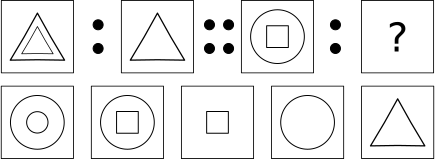
\includegraphics[width=3in]{figures/evans.pdf}
\caption{A geometrical analogy problem: figure $A$ is to figure $B$ as figure
  $C$ is to which candidate?}
\label{FIG:evans}
\end{figure}

The inputs to the program are rough, hand-built low-level descriptions of the
figures. For example, simple geometric shape such as circles, rectangles or
triangles are all described with one single primitive:
\textit{SIMPLE\_CLOSED\_CURVE(\dots)}, where the arguments are the start and
end of of the (multiple) lines, and their curvatures. The program is then
divided into two distinct parts.

The role of the first part is to build high level representations of the
figures from these raw descriptions. After identifying coherent shapes (such as
triangle, square, etc) as independent objects, the program tries to find
relations of the kind \textit{INSIDE(Obj1, Obj2)} or \textit{ABOVE(Obj1, Obj3)}
between figures. Finally, similarities between every pair of objects are
computed. The similarity measure is based on the transformability of the first
object into the second one, using traditional geometrical transformations
(rotation, scale, reflections, etc.). All the information computed by the first
part are given as input (on punched cards!) to the second part.

The second part relates to the analogical solving process per se. Using the
output of the first part, ANALOGY will try to find a set of rules that
transform figure $A$ into figure $B$. A rule would for example state
\textit{REMOVE(Obj1), ROTATE(Obj2, 45\degree), etc.}. Then, by generalizing
each rule, it tries to establish a correspondence between these rules and those
transforming $C$ into one of the candidate solutions. The chosen solution is
the one that maximizes the resemblance between the two sets of rules.

An interesting fact is that ANALOGY analyses the way to go from $A$ to $B$ and
applies it to go from $C$ to $D$, but it does not make use of \textit{central
permutation}\footnote{The central permutation axiom, described in the next
chapter, states that $A:B::C:D \iff A:C::B:D$.}: it may just as well analyze the way to go from $A$ to $C$ and
transpose it to go from $B$ to $D$. Note also that in ANALOGY the semantics
behind the relations and the geometrical objects are not taken into account. In
this respect, ANALOGY is close to Gentner's Structure Mapping Theory (but
preexisting by far).


\subsection{Analogical reasoning as distance minimization on a vector space}
\label{SEC:rumelhart_Abrahamsen}

At a time where most models of analogy used to take the form of complex computer
programs (such as that of Evans), the two cognitive scientists David Rumelhart
and Adele Abrahamsen proposed a simple theoretical model of analogical
reasoning \cite{RumAbr73}. Their model is of great interest for us because as
it will become clear, their view of analogy is in total accordance with our use
of analogy in machine learning (or should we say more humbly that our use of
analogy is fully compliant with their earlier model).

For Rumelhart and Abrahamsen, a human reasoning process can be defined by two
components: a memory structure in which the remembered objects are stored, and
an algorithm that manipulates these data to produce a result. In their paper,
they define these two components for the analogical reasoning.

With regards to the memory structure, their assumption is that it can be
considered as an $m$-dimensional Euclidean space. This assumption is originally
that of Henley \cite{Hen69} who showed, with the help of social experiments,
that a set of 30 mammals could be fairly well represented in the 3-dimensional
space $\mathbb{R}^3$ with the three axes \textit{ferocity}, \textit{humanness},
and \textit{size}. It is supposed that the semantic similarity that people
associate with two concepts is inversely proportional to their distance in the
Euclidean space $\mathbb{R}^3$. For example, \textit{cow} and \textit{horse}
should be fairly close, but \textit{rat} would likely be far from both.

Rumelhart and Abrahamsen are interested in the problem of solving an analogical
equation (although they never state it in these terms): given three concepts
$A, B, C$ and a set of candidate solutions $D_1, D_2, \cdots, D_n$, which $D_i$
is the best candidate for $A:B::C:D_i$? Their assumption is the following:
\textbf{ for a human agent, the best solution is the closest $D_i$ to the
(potentially hypothetical) \textit{perfect} solution $I$, defined as $I = C - A
+ B$}. This principle is illustrated in figure \ref{FIG:rumelhart_model}.
To assess the soundness of this hypothesis, diverse social experiments are led
by the authors. For example, students are asked to choose the best candidates
for various randomly generated analogies, e.g. rat is to pig as goat is to $[$
chimpanzee, cow, rabbit, sheep$]$.

\begin{figure}[!h]
\centering
\includegraphics[width=2.5in]{figures/rumelhart_model.pdf}
  \caption{Analogical equation solving process as in \cite{RumAbr73}. The
  solution is here $D_2$.}
\label{FIG:rumelhart_model}
\end{figure}

As it will become clear, this idea that an analogy $A:B::C:D$ is better when
$D$ is \textbf{close} (as measured by a distance on a metric space) to the true
solution $I$ is entirely compatible with the notion of \textit{analogical
dissimilarity} that will be defined in Chapter \ref{CHAP:functional_definition}.

More recently, various techniques have been proposed to generate a vector-space
embedding for words from a large corpus of text documents, for example
Word2Vect \cite{MikCheCorDea13}. In these continuous spaces also, some
interesting analogies between words can be found that give even more power to
the works of Rumelhart and Abrahamsen. The most classical example of
word-analogy in such a space is given by \textit{man} is to \textit{woman} as
\textit{king} is to \textit{queen}, where the vector
\textit{queen} was found to be the one that is the closest to the vector
\textit{king - man + woman}, which is in perfect accordance to the idea of
Rumelhart and Abrahamsen. Other meaningful analogies can be found, and some of
them are illustrated in Figure \ref{FIG:word_analogies}. See \cite{MikYihZwe13}
for more details on finding linguistic regularities in word space embeddings.
\begin{figure}[!h]
\centering
  \includegraphics[width=5in]{figures/word_analogies.png}
\caption{Analogies between words in the Word2Vect model. Image source:
  \url{https://www.tensorflow.org/versions/master/tutorials/word2vec}.}
  \label{FIG:word_analogies}
\end{figure}


\subsection{The Copycat program}
\label{SEC:copycat}

Copycat \cite{Mit93} (see also \cite{HofMit94}) is another famous program that
performs analogical reasoning tasks, introduced by Melanie Mitchell and Douglas
Hofstadter. The problems considered by Copycat are the solving of analogical
equations in a \textit{microworld} of strings of letters. A typical Copycat
problem looks as follows: $$\mathbf{abc} : \mathbf{abd} :: \mathbf{ijk} : x$$

What should the value of $x$ be? Various answers may be relevant here, such as
$\mathbf{ijd}$ (replace the right-most letter by $\mathbf{d}$), but the most
natural answer probably is $\mathbf{ijl}$: replace the right-most letter by its
successor. How about $\mathbf{zrq}$? Well, not really convincing. The point of
the authors, however, is that \textit{a priori} every single option should be
given equal chances of success.

This principle is strongly reflected in the Copycat program which is
probabilistic in nature: for the same problem, various solutions can be found
depending on the initial condition. For example the  equation $\mathbf{abd} :
\mathbf{abd} :: \mathbf{mrrjjj} : x$ leads to $\mathbf{mrrkkk}$ in 70\% of the
cases (over 1000 experiments), and to $\mathbf{mrjjk}$ 20\% of the time. Other
less plausible solutions make up the remaining 10\%.

At the beginning of the program, each option is equally available.  Then, on
the basis of their validity, some hypotheses are given a stronger chance to
\textit{survive} till the end of the program, while others are discarded.
Conceptually, this process emerges from the interoperability of three main
components: the workspace, the codelets, and the temperature.

\begin{itemize}
    \item The workspace, is the place where objects and relations live.
      In the workspace, diverse conceptual structures are built-in:
      \textit{successor}, \textit{predecessor}, \textit{left-most},
      \textit{right-most}, \textit{orientation}, etc. When the program starts, none of these
      structures are activated: this will be the role of the codelets.
    \item The codelets, are competing agents trying to explore and build
      perceptual structures and relations between the objects in the workspace.
      Their behaviour depends on the temperature.
    \item The temperature could be also defined as the entropy of the
      system. When relations in the workspace are strong and well established,
      the temperature is low. At the beginning of the program, the temperature
      is the highest, leading to a multitude of codelets being run in every
      single \textit{direction}. This concept of temperature can be viewed as
      the trade-off between exploration (trying every possible hypothesis) and
      exploitation (the actual use of a well established hypothesis). When the
      temperature goes below a given threshold, the program stops and the
      current hypothesis is outputted.
\end{itemize}

\begin{figure}[!h]
\centering
  \includegraphics[width=3.5in]{figures/copycat.png}
\caption{Snapshot of Copycat during an equation solving process. Image taken
  from \cite{Mit01}.}
\label{FIG:copycat_snapshot}
\end{figure}

Figure \ref{FIG:copycat_snapshot} illustrate the internal state of Copycat
during the solving of $\mathbf{abc} : \mathbf{abd} :: \mathbf{mrrjjj}: x$. 195
codelets have run so far, so the temperature is average and some structure have
been properly established, such as the \textit{successor group} $\mathbf{abc}$
and the \textit{sameness group} $\mathbf{jjj}$. The $\mathbf{rr}$ group is also
begin defined, though still weaker than the others at this stage. Also, a rule
describing the change from $\mathbf{abc}$ to $\mathbf{abd}$ has been
established: \textit{replace the right-most letter by its successor}. Depending
on the future behaviour of the codelets, this rule with either stick till the
end of the program or change to lead to the most common prediction $x =
\mathbf{kkk}$.

Copycat is clearly a complex adaptative system where a global behaviour emerges
from small, independent parts. According to its authors, \textit{Copycat's
architecture is neither symbolic nor connectionist, nor a hybrid of the two;
rather, the program has a novel type of architecture situated somewhere in
between these extremes}.

\subsection{Analogy and the Minimum Description Length Principle}

Ockham's razor (also Occam), due to the Franciscan philosopher William
of Ockham (1285~-~1347), is a well known principle in machine learning theory.
The main and most useful interpretation of the original Latin version states
that when trying to explain a situation, if two hypothesis give the same answer
then the best one is probably the \textbf{simplest} one. In practice, what
makes an hypothesis simple remains quite vague, at least from a computational
point of view. Yet this principle has been formalized into Rissanen's Minimum
Description Length Principle (MDLP) \cite{Ris78}, which is based on Kolmogorov
complexity. Despite the difficulty to build inferential models from this
principle (Kolmogorov complexity is often intractable and impossible to
compute, and can only be estimated), it has shown to be quite influential in
the field of machine learning, at least from a theoretical point of view.

With this in mind, Antoine Cornuéjols proposed a framework for assessing the
quality of an analogy \cite{CorMLS96} (see also \cite{CorJFA96}). In these
papers, Cornuéjols hypothesizes that the best analogy between a source and a
target model is the \textit{simplest} one, meaning that its description length
is minimal, in terms of Kolmogorov complexity.

Let us first first recall some basic knowledge about Kolmogorov complexity,
before diving into more technical details. The Kolmogorov complexity of a
string of characters $x$, denoted $K(x)$, is the length of the shortest
computer program capable of outputting $x$ on a universal Turing machine. $K(x)$ is supposed to capture the
intrinsic complexity of $x$. Intuitively, $K('aaaaabbbbb')$ is supposed to be
lower than $K('abaabbabab')$, because a clear pattern emerges in the first
string, leading to a simple program: first print $a$ five times, then do the
same for $b$. The second string seems more or less random, which makes it
difficult to factorize into a concise program. In some sense, the Kolmogorov
complexity captures how well a string $x$ can be \textit{compressed}. The
conditional complexity $K(x \given y)$ is the size of the shortest program that
outputs $x$ when given $y$ as an input.

Now, let's get back to our analogical concerns. As illustrated in figure
\ref{FIG:cornuejols_model}, Cornuéjols considers an analogy as a process
involving an object $x_S$ in a source domain, an object $x_T$ in a target
domain, and two functions $f_S$ and $f_T$ transforming $x_S$ and $x_T$ into
$y_S$ and $y_T$ respectively: $y_S = f_S(x_S)$ and $y_T = f_T(x_T)$. Each
domain $S$ and $T$ \textit{lives} inside a theory or model (namely $M_S$ and
$M_T$), that can describe their corresponding objects.

\begin{figure}[!h]
\centering
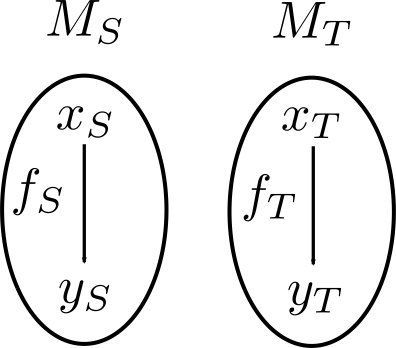
\includegraphics[width=1.5in]{figures/cornuejols_model.pdf}
\caption{The two domains $S$ and $T$ in Cornuejols' model.}
\label{FIG:cornuejols_model}
\end{figure}

For Cornuéjols, the best analogy is the one that minimizes the following sum of
Kolmogorov complexities:
$$K(M_S) + K(x_S \given M_S) + K(f_S \given M_S) + K(M_T \given M_S) + K(x_T
\given M_T) + K(f_T \given M_T),$$
where:
\begin{itemize}
   \item $K(M_S)$ is the cost associated with the source theory,
   \item $K(x_S \given M_S)$ is the cost of $x_S$ as described in the source
     theory,
   \item $K(f_S \given M_S)$ is the cost of $f_S$ as described in the source
     theory,
   \item $K(M_T \given M_S)$ is the cost of describing the target theory from
     the source theory,
   \item $K(x_T \given M_T)$ is the cost of $x_T$ as described in the target
     theory,
   \item and finally $K(f_T \given M_T)$ is the cost of $f_T$ as described in
     the target theory.
\end{itemize}

Notice that the terms $y_i$ are not considered in this cost function, because
they are entirely defined by their corresponding $x_i$ and $f_i$.

Cornuéjols illustrate the plausibility of his model using experiments in the
microworld of Copycat. After defining the Kolmogorov complexity of the built-in
relations (\textit{direction}, \textit{length}, etc.), and those of the
representations of the inputs, the solutions of the analogical equations are
set as those minimizing the above criterion. The empirical results show that
this model, in addition to its theoretical appeal due to the proximity with
MDLP, is at the very least an interesting option that deserves further
investigations. In a
recent work , this model of analogy has been applied to a task of transfer
learning \cite{CorMur16}.

Adopting a different (but close) approach, the association between Kolmogorov
complexity and the evaluation of the quality of an analogy has also been
recently advocated in \cite{BayPraRic12}. In this work, the authors propose
that if four objects $a, b, c, d$ are in proportion, then it should be as
\textit{complicated} to go from $a$ to $b$ as to go from $c$ to $d$, and it
should also be as \textit{complicated} to go from $b$ to $a$ as to go from $d$
to $c$. More formally:
$$a:b::c:d \implies K(b \given a) = K(d \given c) \text{ and } K(a \given b) =
K(c \given d).$$
This criterion was used to automatically discriminate \textit{good} analogies
from \textit{bad} analogies, where objects were concepts represented as words
of the natural language, and where their Kolmogorov complexity was roughly
approximated using online search-engine queries. The experiments showed that
the system was able to differentiate credible analogies from fishy ones in
about 75\% of the time.

\subsection{Case-Based Reasoning}

We will here describe the field of Case-Based Reasoning (CBR). First of all,
let us note that CBR is not literally a computational model of analogy, but is
rather a general problem solving paradigm that makes use of some particular
form of analogical reasoning. As discussed in \cite{AamPla94}, CBR and
analogical reasoning are often mixed up in the literature.  We choose to
briefly describe CBR now, because we need to clarify how our approach to
problem solving will differ from that of CBR.

CBR is a very general paradigm for problem solving, where a new problem is
solved using the knowledge of some similar past experiences. This model can be
motivated by its psychological appeal: it is indeed well acknowledged that,
when confronted with an unknown situation, humans tend to make use of their
past knowledge about some other similar situation to solve the problem at hand.
As an example, the recipe of a strawberry pie could be easily inferred using
the past knowledge on the recipe of other fruit-pies (e.g. apple pie, pear pie,
etc.).

In its most general form, CBR is a way of reaching the unknown solution $S$ to a
problem $P$ using the known solutions $S_i$ to problems $P_i$ that are
\textbf{similar} to $P$. Each couple $(S_i, P_i)$ is called a \textbf{case},
hence the name of the paradigm.  The term \textit{problem} is here used in its
most general sense.  In \cite{AamPla94}, a CBR process is described by the
succession of the following four steps:
\begin{enumerate}
  \item \textbf{Retrieve}: this first step is to retrieve all cases $(S_i,
    P_i)$ where $P_i$ is similar to the initial problem $P$. The way these
    cases are chosen is entirely dependent of the current setting, and greatly
    differ depending on the application. Sometimes, only a single case  is
    selected.
  \item \textbf{Reuse}: the solutions $S_i$ associated to the most relevant
    $P_i$ are aggregated in some way, and adapted if needed to build up the
    final solution $S$.
  \item \textbf{Revise}: the relevance and the adequacy of the chosen solution
    $S$ is evaluated, and $S$ is modified if needed.
  \item \textbf{Retain}: if the revised solution $S$ ended up being a good
    choice, then the solution is retained and the couple $(P, S)$ is bound to
    be used in the solving of some future problems.
\end{enumerate}

%%Quite amusingly, the CBR community tends to see analogical reasoning as a
%%subfield of CBR, while the analogical reasoning community seems to believe that
%%CBR is a particular instance of analogy-based reasoning. Indeed in
%%\cite{AamPla94}, the authors (that are CBR oriented) define analogical
%%reasoning as a particular CBR instance that is focused on solving cross-domain
%%problems, i.e. where a problem in a source domain has to be mapped into a
%%problem in a target domain. While this description of analogical reasoning is
%%fairly reasonable, one may object that what defines the source and target
%%domains is completely arbitrary, thus reducing CBR to a particular instance of
%%analogical reasoning where the source and target domains are forced to be the
%%same.
%%
%%We will not further discuss this point here but

Before moving further to the next chapter, we would like to point out a
significant difference between the CBR approach and the one we will address in
this document. In a way, the CBR process can be viewed as building the
following analogical proportions:
$$P_i:S_i :: P : S, $$
where $S$ is unknown and inferred from all the $S_i$. We can indeed consider
that \textit{problem $P_i$ is to solution $S_i$ as problem $P$ is to solution
$S$}. Each of these analogical proportions is built on the basis that $P_i$ and
$P$ are \textbf{similar}, so $S$ should be similar to $S_i$.

But as we will see in the next chapter, an analogical proportion $a:b::c:d$ is
not restricted to having $a$ close to $c$ and $b$ close to $d$! It is quite the
contrary actually: all elements are allowed to be extremely distinct. And
indeed, if we are able to \textit{capture} how a given $P_i$ (that is not close
to $P$) differs from $P$, then applying the same transformation to $S_i$ should
give us a relevant potential solution $S$.  Acknowledging this fact, our
approach to analogical learning will rather follow the following conceptual
scheme: we will try to retrieve the proportions of the form $P_{i_1} : P_{i_2}
:: P_{i_3} : P$, and the solution $S$ will be inferred by
\textit{extrapolation}\footnote{The way $S$ is \textit{extrapolated} will be
described in the next chapter as the \textbf{solving} of the analogical
equation.} from the associated equations: $S_{i_1} : S_{i_2} :: S_{i_3} :
S$. This allows us to consider problems $P_i$ that are both similar
\textbf{and} different from $P$, which may allow to find more interesting
solutions $S$.

\section*{Conclusion}

This first chapter was devoted to the description of past works on the modeling
of analogical reasoning. We chose here to distinguish between two groups of
models: those that make explicit use of analogical proportions (either as a key
component of the model or as a simple use-case example), and those that do not.
Among the models that use analogical proportions, we will see that the model
of Rumelhart and Abrahamsen (derived from a psychological perspective) will be
in perfect accordance to our view of analogical classification, and analogical
learning in general.

It is fairly clear that these past works are, with a few exceptions, mostly
motivated by cognitive and psychological investigations. It is only recently
that some authors, starting from the pioneering investigation in \cite{Lep04},
have provided a formal framework to deal with analogical proportions in general
algebraic settings, which opened the door to many computational applications.
These formal analogical proportions probably are the most important concept of
this document. We will now review this topic in the next chapter.
